\documentclass[12pt,a4paper]{article}
\usepackage[UTF8]{ctex}
\usepackage{amsmath,amssymb}
\usepackage{listings}
\usepackage{xcolor}
\usepackage{hyperref}
\usepackage{geometry}
\usepackage{graphicx}
\geometry{margin=2.5cm}

\lstdefinestyle{python}{
  language=Python,
  basicstyle=\ttfamily\small,
  keywordstyle=\color{blue}\bfseries,
  commentstyle=\color{gray},
  stringstyle=\color{red},
  showstringspaces=false,
  breaklines=true,
  frame=single,
  backgroundcolor=\color{gray!10}
}

\title{Bit Flip Code / 比特翻转码}
\author{QuoNic}
\date{}

\begin{document}
\maketitle

\begin{center}
\textbf{Error Correction / 纠错} | 难度：初级 | 预计时间：10 分钟
\end{center}

\tableofcontents
\newpage

\section{为什么需要？}

量子比特容易受噪声影响，比特翻转码是最简单的量子纠错码。

\subsection{经典局限}
\begin{itemize}
  \item 量子比特无法复制（不可克隆定理）
  \item 量子测量会破坏量子态
  \item 经典纠错码不能直接用于量子系统
\end{itemize}

\subsection{量子优势}
\begin{itemize}
  \item 比特翻转码用 3 个物理量子比特编码 1 个逻辑量子比特
  \item 可以检测和纠正单比特翻转错误
  \item 是量子纠错的基础
\end{itemize}

\subsection{实际应用}
\begin{itemize}
  \item 量子计算（纠错）
  \item 量子通信（保护量子态）
  \item 量子存储（延长相干时间）
\end{itemize}

\section{快速上手}

\begin{lstlisting}[style=python]
from quonic.qec import bit_flip_code

# Encode, introduce error, correct
result = bit_flip_code(error_qubit=1)
print(f"Original: {result.original}")
print(f"Corrected: {result.corrected}")
\end{lstlisting}

\textbf{预期输出}：
\begin{verbatim}
Original: |0>
Corrected: |0>
\end{verbatim}

\section{原理详解}

\subsection{电路图}

\begin{center}
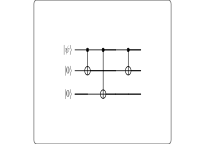
\includegraphics[width=0.7\textwidth]{../../images/bit_flip_code_circuit.svg}
\end{center}

\subsection{数学推导}

\textbf{编码}：
\begin{equation}
|0\rangle \to |000\rangle, \quad |1\rangle \to |111\rangle
\end{equation}

\textbf{错误}：如果 $q_1$ 发生翻转：
\begin{equation}
|000\rangle \to |010\rangle
\end{equation}

\textbf{纠正}：通过多数投票恢复：
\begin{equation}
|010\rangle \to |000\rangle
\end{equation}

\subsection{几何解释}

比特翻转码将量子态冗余编码到 3 个量子比特中。即使一个量子比特发生错误，通过多数投票可以恢复原始态。

\section{代码详解}

\begin{lstlisting}[style=python]
from quonic.qec import bit_flip_code

# bit_flip_code(error_qubit)
# error_qubit: which qubit has the error (None for no error)
result = bit_flip_code(error_qubit=1)

# result.original: original state
# result.encoded: encoded state
# result.error: state after error
# result.corrected: corrected state
print(f"Corrected: {result.corrected}")
\end{lstlisting}

\section{进阶用法}

\subsection{场景 1：不同错误位置}

\begin{lstlisting}[style=python]
# Error on different qubits
for i in range(3):
    result = bit_flip_code(error_qubit=i)
    print(f"Error on q{i}: {result.corrected}")
\end{lstlisting}

\subsection{场景 2：无错误}

\begin{lstlisting}[style=python]
# No error
result = bit_flip_code(error_qubit=None)
print(f"No error: {result.corrected}")
\end{lstlisting}

\section{适用场景}

\subsection{量子计算}

比特翻转码是量子纠错的基础构建块。

\subsection{量子通信}

比特翻转码可以保护量子通信中的量子态。

\subsection{量子存储}

比特翻转码可以延长量子存储的相干时间。

\section{常见问题}

\subsection{比特翻转码能纠正所有错误吗？}

不能。比特翻转码只能纠正单比特翻转错误，不能纠正相位错误。

\subsection{比特翻转码需要多少量子比特？}

需要 3 个物理量子比特编码 1 个逻辑量子比特。

\subsection{比特翻转码和相位翻转码有什么区别？}

比特翻转码纠正 $X$ 错误（翻转），相位翻转码纠正 $Z$ 错误（相位）。

\section{学习路径}

\subsection{前置知识}
\begin{itemize}
  \item 量子比特和量子门
  \item 量子测量
  \item 量子噪声
\end{itemize}

\subsection{继续学习}
\begin{itemize}
  \item 相位翻转码
  \item Shor 码（9 量子比特）
  \item 表面码
\end{itemize}

\section{完整示例代码}

\subsection{示例 1：基本比特翻转码}

\begin{lstlisting}[style=python]
from quonic.qec import bit_flip_code

result = bit_flip_code(error_qubit=1)
print(f"Corrected: {result.corrected}")
\end{lstlisting}


\section{下载}

\begin{itemize}
  \item [bit_flip_code.py](https://github.com/ChrisLee0721/QuoNic/blob/main/examples/bit_flip_code/bit_flip_code.py)
\end{itemize}

\end{document}
